\documentclass[a4paper,twoside]{article}

\usepackage{epsfig}
\usepackage{graphicx} 
\usepackage{subcaption}
\usepackage{calc}
\usepackage{amssymb}
\usepackage{amstext}
\usepackage{amsmath}
\usepackage{amsthm}
\usepackage{multicol}
\usepackage{pslatex}
\usepackage{apalike}
\usepackage{algorithm2e}
\usepackage[bottom]{footmisc}
\usepackage{SCITEPRESS}     % Please add other packages that you may need BEFORE the SCITEPRESS.sty package.
\usepackage{siunitx}
\usepackage{booktabs}
\usepackage{threeparttable}

\begin{document}

\title{Solving the Capacitated Vehicle Routing Problem with Dynamic Graph Transformers}

\author{\authorname{Evgeny Polyachenko Name\sup{1}\orcidAuthor{0000-0000-0000-0000}, Second Author Name\sup{1}\orcidAuthor{0000-0000-0000-0000} and Third Author Name\sup{2}\orcidAuthor{0000-0000-0000-0000}}
\affiliation{\sup{1}2Interdisciplinary Centre for Security, Reliability and Trust, University of Luxembourg, Luxembourg}
\affiliation{\sup{2}Department of Computing, Main University, MySecondTown, MyCountry}
\email{\{first\_author, second\_author\}@ips.xyz.edu, evgeny.polyachenko@uni.lu}
}

\keywords{The paper must have at least one keyword. The text must be set to 9-point font size and without the use of bold or italic font style. For more than one keyword, please use a comma as a separator. Keywords must be titlecased.}

\abstract{This paper presents a novel approach to solving the Capacitated Vehicle Routing Problem (CVRP) using Dynamic Graph Transformers. We leverage the power of deep reinforcement learning to train an agent that can dynamically construct high-quality routes for a fleet of vehicles. Our model is evaluated on a set of well-known CVRP benchmarks, and we show that it outperforms existing methods in terms of both solution quality and computational time.}




\onecolumn \maketitle \normalsize \setcounter{footnote}{0} \vfill

\section{\uppercase{Introduction}}
\label{sec:introduction}

\section{Model settings}

\subsection{Instances}

\subsection{GAT}


\subsection{GT}


\section{Optimal and suboptimal benchmarks}

\begin{figure*}[t!]
\centering
   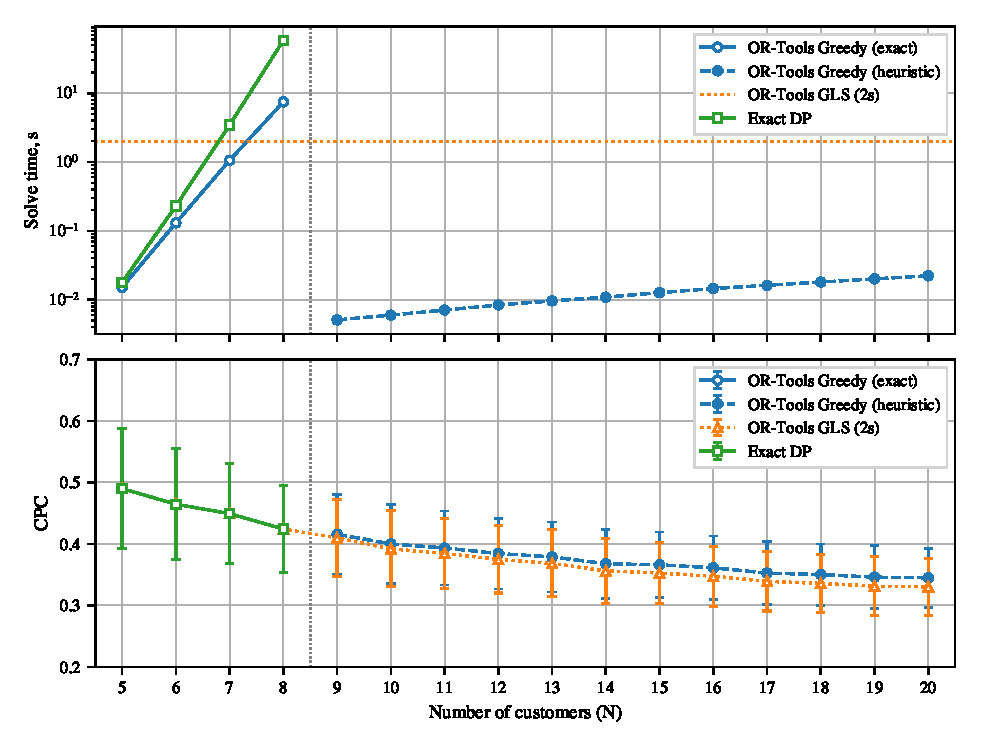
\includegraphics[width=160mm]{figures/benchmark.eps}
   \caption{Performance comparison of CVRP solvers on CPU benchmarks. 
       \textbf{Top panel:} Solve time (log scale) versus problem size for different solvers. 
       Exact DP provides optimal solutions but is limited to small instances (N$\leq$8). 
       OR-Tools Greedy operates in exact mode for N$\leq$8 (solid line) and switches to heuristic mode for larger instances (dashed line). 
       OR-Tools GLS with 2-second time limit maintains consistent performance across all problem sizes (dotted line). 
       \textbf{Bottom panel:} Cost per customer (CPC) showing solution quality with error bars indicating standard deviation across 1000 instances per problem size. 
       The vertical line at N=8.5 marks the transition point between exact and heuristic approaches for OR-Tools Greedy.}
\label{fig:benchmark}
% trim={5pt 10pt 5pt 8pt}, clip
\end{figure*}


\begin{figure}[t!]
\centering
   \includegraphics[width=85mm]{figures/log_norm_N10.eps}
   \caption{Distribution of log(CPC) for N=10 CVRP instances solved using GPU dynamic programming. The histogram shows 100,000 random instances with the fitted normal distribution overlaid ($\mu=-0.748$, $\sigma=0.183$). The log-normal fit demonstrates that CPC follows a log-normal distribution (Kolmogorov-Smirnov test, $p=0.189$).}
\label{fig:benchmark}
% trim={5pt 10pt 5pt 8pt}, clip
\end{figure}


\begin{table*}[htbp]
\centering
\caption{GPU CVRP Performance with Log-normal Statistics and Normality Tests}
\label{tab:gpu-performance-complete}
\begin{tabular}{@{}l c c S[table-format=1.4] S[table-format=1.4] c c c c c c@{}}
\toprule
\textbf{Method} & \textbf{N} & \textbf{Cap.} & {\textbf{GM}} & {\textbf{GSD}} & 
\textbf{95\% Range} & \textbf{95\% CI} & \textbf{KS} & \textbf{D'Agost.} & \textbf{JB} & \textbf{AD} \\
\midrule
Exact (100k) & 10 & 20 & 0.4735 & 1.2012 & [0.3306, 0.6782] & [0.4730, 0.4741] & $0.19$ & $<$0.001 & $<$0.001 & $1.405^*$ \\
Exact (10k) & 10 & 20 & 0.4737 & 1.1996 & [0.3316, 0.6767] & [0.4720, 0.4754] & $0.93$ & $0.37$ & $0.37$ & $0.295$ \\
Heuristic & 10 & 20 & 0.4831 & 1.2064 & [0.3344, 0.6978] & [0.4813, 0.4849] & $0.87$ & $0.44$ & $0.44$ & $0.353$ \\
Heuristic* & 20 & 30 & 0.3319 & 1.1514 & [0.2518, 0.4376] & [0.3310, 0.3328] & $1.00$ & $0.85$ & $0.86$ & $0.093$ \\
Heuristic* & 50 & 40 & 0.2303 & 1.1291 & [0.1815, 0.2921] & [0.2297, 0.2308] & $0.73$ & $0.29$ & $0.28$ & $0.400$ \\
OR-Tools GLS & 100 & 50 & 0.1811 & 1.1058 & [0.1487, 0.2206] & [0.1776, 0.1847] & $0.47$ & $0.39$ & $0.49$ & $0.521$ \\
\bottomrule
\end{tabular}
\begin{tablenotes}
\small
\item GM: Geometric Mean, GSD: Geometric Standard Deviation
\item 95\% Range: Individual value range GM $\times$ [GSD$^{-1.96}$, GSD$^{+1.96}$]
\item 95\% CI: Confidence interval for the geometric mean
\item KS: Kolmogorov-Smirnov, D'Agost.: D'Agostino, JB: Jarque-Bera (p-values for log(CPC) normality)
\item AD: Anderson-Darling test statistic (critical value at 5\% = 0.787; * indicates rejection)
\item * Based on partial benchmark data from GPU heuristic
\item OR-Tools GLS: 100 instances with 1s time limit per instance
\end{tablenotes}
\end{table*}



\begin{table*}[htbp]
\centering
\caption{GPU Improved Heuristic Performance (10,000 instances)}
\label{tab:gpu-heuristic-10000}
\begin{tabular}{@{}c c S[table-format=1.4] S[table-format=1.4] S[table-format=1.4] c@{}}
\toprule
\textbf{N} & \textbf{Capacity} & {\textbf{Mean CPC}} & {\textbf{Std CPC}} & {\textbf{SEM}} & \textbf{2×SEM/Mean(\%)} \\
\midrule
 10 & 20 & 0.4815 & 0.0886 & 0.0003 & 0.12\% \\ %exact-dp 100k
 10 & 20 & 0.4816 & 0.0881 & 0.0008 & 0.37\% \\ %exact-dp 
 10 & 20 & 0.4916 & 0.0929 & 0.0009 & 0.38\% \\
 20 & 30 & 0.3353 & 0.0476 & 0.0005 & 0.28\% \\
 50 & 40 & 0.2316 & 0.0283 & 0.0003 & 0.24\% \\
100 & 50 & 0.1753 & 0.0208 & 0.0002 & 0.24\% \\
\bottomrule
\end{tabular}
\end{table*}




Your paper will be part of the conference proceedings
therefore we ask that authors follow the guidelines explained in
this example in order to achieve the highest quality possible
\cite{Smith98}.

Be advised that papers in a technically unsuitable form will be
returned for retyping. After returned the manuscript must be
appropriately modified.

\section{\uppercase{Manuscript Preparation}}

We strongly encourage authors to use this document for the
preparation of the camera-ready. Please follow the instructions
closely in order to make the volume look as uniform as possible
\cite{Moore99}.

Please remember that all the papers must be in English and without
orthographic errors.

Do not add any text to the headers (do not set running heads) and
footers, not even page numbers, because text will be added
electronically.

For a best viewing experience the used font must be Times New
Roman, except on special occasions, such as program code
\ref{subsubsec:program_code}.


\subsection{Manuscript Setup}

The template is composed by a set of 7 files, in the
following 2 groups:\\
\noindent {\bf Group 1.} To format your paper you will need to copy
into your working directory, but NOT edit, the following 4 files:
\begin{verbatim}
  - apalike.bst
  - apalike.sty
  - article.cls
  - scitepress.sty
\end{verbatim}

\noindent {\bf Group 2.} Additionally, you may wish to copy and edit
the following 3 example files:
\begin{verbatim}
  - example.bib
  - example.tex
  - scitepress.eps
\end{verbatim}


\subsection{Page Setup}

The paper size must be set to A4 (210x297 mm). The document
margins must be the following:

\begin{itemize}
    \item Top: 3,3 cm;
    \item Bottom: 4,2 cm;
    \item Left: 2,6 cm;
    \item Right: 2,6 cm.
\end{itemize}

It is advisable to keep all the given values because any text or
material outside the aforementioned margins will not be printed.


\subsection{First Section}

This section must be in one column.

\subsubsection{Title and Subtitle}

Use the command \textit{$\backslash$title} and follow the given structure in "example.tex". The title and subtitle must be with initial letters
capitalized (titlecased). The separation between the title and subtitle is done by adding a colon ":" just before the subtitle beginning. In the title or subtitle, words like "is", "or", "then", etc. should not be capitalized unless they are the first word of the title or subtitle. No formulas or special characters of any form or language are allowed in the title or subtitle.

\subsubsection{Authors and Affiliations}

Use the command \textit{$\backslash$author} and follow the given structure in "example.tex". Please note that the name of each author must start with its first name.

\subsubsection{Keywords}

Use the command \textit{$\backslash$keywords} and follow the given structure in "example.tex". Each paper must have at least one keyword. If more than one is specified, please use a comma as a separator. The sentence must end with a period.

\subsubsection{Abstract}

Use the command \textit{$\backslash$abstract} and follow the given structure in "example.tex".
Each paper must have an abstract up to 200 words. The sentence
must end with a period.

\subsection{Second Section}

Files "example.tex" and "example.bib" show how to create a paper
with a corresponding list of references.

This section must be in two columns.

Each column must be 7,5-centimeter wide with a column spacing
of 0,8-centimeter.

The section text must be set to 10-point.

Section, subsection and sub-subsection first paragraph should not
have the first line indent.

To remove the paragraph indentation (only necessary for the
sections), use the command \textit{$\backslash$noindent} before the
paragraph first word.

If you use other style files (.sty) you MUST include them in the
final manuscript zip file.


\subsubsection{Section Titles}

The heading of a section title should be in all-capitals.

Example: \textit{$\backslash$section\{FIRST TITLE\}}

\subsubsection{Subsection Titles}

The heading of a subsection title must be with initial letters
capitalized (titlecased).

Words like "is", "or", "then", etc. should not be capitalized unless
they are the first word of the subsection title.

Example: \textit{$\backslash$subsection\{First Subtitle\}}

\subsubsection{Sub-Subsection Titles}

The heading of a sub subsection title should be with initial letters
capitalized (titlecased).

Words like "is", "or", "then", etc should not be capitalized unless
they are the first word of the sub subsection title.

Example: \textit{$\backslash$subsubsection\{First Subsubtitle\}}

\subsubsection{Tables}

Tables must appear inside the designated margins or they may span
the two columns.

Tables in two columns must be positioned at the top or bottom of the
page within the given margins. To span a table in two columns please add an asterisk (*) to the table \textit{begin} and \textit{end} command.

Example: \textit{$\backslash$begin\{table*\}}

\hspace*{1.5cm}\textit{$\backslash$end\{table*\}}\\

Tables should be centered and should always have a caption
positioned above it. The font size to use is 9-point. No bold or
italic font style should be used.

The final sentence of a caption should end with a period.

\begin{table}[h]
\caption{This caption has one line so it is
centered.}\label{tab:example1} \centering
\begin{tabular}{|c|c|}
  \hline
  Example column 1 & Example column 2 \\
  \hline
  Example text 1 & Example text 2 \\
  \hline
\end{tabular}
\end{table}

\begin{table}[h]
\vspace{-0.2cm}
\caption{This caption has more than one line so it has to be
justified.}\label{tab:example2} \centering
\begin{tabular}{|c|c|}
  \hline
  Example column 1 & Example column 2 \\
  \hline
  Example text 1 & Example text 2 \\
  \hline
\end{tabular}
\end{table}

Please note that the word "Table" is spelled out.


\subsubsection{Figures}

Please produce your figures electronically, and integrate them into
your document and zip file.

Check that in line drawings, lines are not interrupted and have a
constant width. Grids and details within the figures must be clearly
readable and may not be written one on top of the other.

Figure resolution should be at least 300 dpi.

Figures must appear inside the designated margins or they may span
the two columns.

Figures in two columns must be positioned at the top or bottom of
the page within the given margins. To span a figure in two columns please add an asterisk (*) to the figure \textit{begin} and \textit{end} command.

Example: \textit{$\backslash$begin\{figure*\}}

\hspace*{1.5cm}\textit{$\backslash$end\{figure*\}}

Figures should be centered and should always have a caption
positioned under it. The font size to use is 9-point. No bold or
italic font style should be used.


The final sentence of a caption should end with a period.



Please note that the word "Figure" is spelled out.

\subsubsection{Equations}

Equations should be placed on a separate line, numbered and
centered.\\The numbers accorded to equations should appear in
consecutive order inside each section or within the contribution,
with the number enclosed in brackets and justified to the right,
starting with the number 1.

Example:

\begin{equation}\label{eq1}
    a=b+c
\end{equation}

\subsubsection{Algorithms and Listings}

Algorithms and Listings captions should have font size 9-point, no bold or
italic font style should be used and the final sentence of a caption should end with a period. The separator between the title of algorithms/listings and the name of the algorithm/listing must be a colon.
Captions with one line should be centered and if it has more than one line it should be set to justified.

\begin{algorithm}[!h]
 \caption{How to write algorithms.}
 \KwData{this text}
 \KwResult{how to write algorithm with \LaTeX2e }
 initialization\;
 \While{not at end of this document}{
  read current\;
  \eIf{understand}{
   go to next section\;
   current section becomes this one\;
   }{
   go back to the beginning of current section\;
  }
 }
\end{algorithm}


\bigskip
\subsubsection{Program Code}\label{subsubsec:program_code}

Program listing or program commands in text should be set in
typewriter form such as Courier New.

Example of a Computer Program in Pascal:

\begin{small}
\begin{verbatim}
 Begin
     Writeln('Hello World!!');
 End.
\end{verbatim}
\end{small}


The text must be aligned to the left and in 9-point type.

\subsubsection{Reference Text and Citations}

References and citations should follow the APA (Author, date)
System Convention (see the References section in the compiled
manuscript). As example you may consider the citation
\cite{Smith98}. Besides that, all references should be cited in the
text. No numbers with or without brackets should be used to list the
references.

References should be set to 9-point. Citations should be 10-point
font size.

You may check the structure of "example.bib" before constructing the
references.

For more instructions about the references and citations usage
please see the appropriate link at the conference website.

\section{\uppercase{Copyright Form}}

For the mutual benefit and protection of Authors and
Publishers, it is necessary that Authors provide formal written
Consent to Publish and Transfer of Copyright before publication of
the Book. The signed Consent ensures that the publisher has the
Author's authorization to publish the Contribution.

The copyright form is located on the authors' reserved area.

The form should be completed and signed by one author on
behalf of all the other authors.

\section{\uppercase{Conclusions}}
\label{sec:conclusion}

Please note that ONLY the files required to compile your paper should be submitted. Previous versions or examples MUST be removed from the compilation directory before submission.

We hope you find the information in this template useful in the preparation of your submission.


\section*{\uppercase{Acknowledgements}}

If any, should be placed before the references section
without numbering. To do so please use the following command:
\textit{$\backslash$section*\{ACKNOWLEDGEMENTS\}}


\bibliographystyle{apalike}
{\small
\bibliography{example}}


\section*{\uppercase{Appendix}}

If any, the appendix should appear directly after the
references without numbering, and not on a new page. To do so please use the following command:
\textit{$\backslash$section*\{APPENDIX\}}

\end{document}


\begin{table*}[htbp]
\centering
\caption{OR-Tools Greedy Heuristic Performance (PATH\_CHEAPEST\_ARC Strategy)}
\label{tab:ortools-greedy}
\begin{tabular}{@{}c c c S[table-format=1.6] S[table-format=1.6] S[table-format=1.6] c@{}}
\toprule
\textbf{N} & \textbf{Capacity} & \textbf{Instances} & {\textbf{Mean CPC}} & {\textbf{Std CPC}} & {\textbf{SEM}} & \textbf{2×SEM/Mean(\%)} \\
\midrule
10  & 20 & 10 & 0.4557 & 0.0718 & 0.0227 & 9.97\% \\
20  & 30 & 10 & 0.3389 & 0.0398 & 0.0126 & 7.43\% \\
50  & 40 & 10 & 0.2515 & 0.0274 & 0.0087 & 6.90\% \\
100 & 50 & 10 & 0.1801 & 0.0188 & 0.0059 & 6.59\% \\
\bottomrule
\end{tabular}
\end{table*}

% Table 2: OR-Tools GLS (GUIDED_LOCAL_SEARCH)
\begin{table*}[htbp]
\centering
\caption{OR-Tools Guided Local Search Performance (GUIDED\_LOCAL\_SEARCH Metaheuristic)}
\label{tab:ortools-gls}
\begin{tabular}{@{}c c c S[table-format=1.6] S[table-format=1.6] S[table-format=1.6] c@{}}
\toprule
\textbf{N} & \textbf{Capacity} & \textbf{Instances} & {\textbf{Mean CPC}} & {\textbf{Std CPC}} & {\textbf{SEM}} & \textbf{2×SEM/Mean(\%)} \\
\midrule
10  & 20 & 10 & 0.4481 & 0.0708 & 0.0224 & 10.00\% \\
20  & 30 & 10 & 0.3245 & 0.0324 & 0.0102 & 6.32\% \\
50  & 40 & 10 & 0.2433 & 0.0276 & 0.0087 & 7.18\% \\
100 & 50 & 10 & 0.1776 & 0.0197 & 0.0062 & 7.02\% \\
\bottomrule
\end{tabular}
\end{table*}


10  & 20 & 0.4481 & 0.0708
20  & 30 & 0.3245 & 0.0324
50  & 40 & 0.2433 & 0.0276
100 & 50 & 0.1776 & 0.0197


\begin{table*}[htbp]
\centering
\caption{GPU Improved Heuristic Performance (100 instances)}
\label{tab:gpu-heuristic-100}
\begin{tabular}{@{}c c S[table-format=1.4] S[table-format=1.4] S[table-format=1.4] c@{}}
\toprule
\textbf{N} & \textbf{Capacity} & {\textbf{Mean CPC}} & {\textbf{Std CPC}} & {\textbf{SEM}} & \textbf{2×SEM/Mean(\%)} \\
\midrule
 10 & 20 & 0.4731 & 0.0834 & 0.0083 & 3.53\% \\ % exact-dp
 10 & 20 & 0.4845 & 0.0916 & 0.0092 & 3.78\% \\
 20 & 30 & 0.3367 & 0.0449 & 0.0045 & 2.67\% \\
 50 & 40 & 0.2317 & 0.0266 & 0.0027 & 2.30\% \\
100 & 50 & 0.1751 & 0.0169 & 0.0017 & 1.94\% \\
\bottomrule
\end{tabular}
\end{table*}


\begin{table*}[htbp]
\centering
\caption{GPU Improved Heuristic Performance (1,000 instances)}
\label{tab:gpu-heuristic-1000}
\begin{tabular}{@{}c c S[table-format=1.4] S[table-format=1.4] S[table-format=1.4] c@{}}
\toprule
\textbf{N} & \textbf{Capacity} & {\textbf{Mean CPC}} & {\textbf{Std CPC}} & {\textbf{SEM}} & \textbf{2×SEM/Mean(\%)} \\
\midrule
 10 & 20 & 0.4824 & 0.0904 & 0.0029 & 1.19\% \\ %exact-dp
 10 & 20 & 0.4932 & 0.0961 & 0.0030 & 1.23\% \\
 20 & 30 & 0.3388 & 0.0468 & 0.0015 & 0.87\% \\
 50 & 40 & 0.2312 & 0.0280 & 0.0009 & 0.77\% \\
100 & 50 & 0.1761 & 0.0205 & 0.0006 & 0.73\% \\
\bottomrule
\end{tabular}
\end{table*}
